\def \ti{\textit}
\def \bf{\textbf}

\chapter{Progettazione}
	\label{cap:progettazione}
	
    In questo capitolo verranno analizzate in dettaglio le scelte progettuali che hanno permesso la realizzazione del sistema software. Dopodiché si analizzerà, attraverso la rappresentazione dei diagrammi \textbf{UML}, la definizione delle fasi di sviluppo, ossia la progettazione delle funzionalità correnti dell'applicazione.

\section{Requisiti}
	\label{sec:requisiti}
	Come primo aspetto della progettazione si analizzeranno adesso i requisiti del sistema. Innanzitutto si deve specificare che l'intero sistema è pensato per essere utilizzato in un ambito amministrativo dove gli utenti possono essere per esempio i dipendenti di un'azienda. Questo vuol dire che ci si trova in un sistema chiuso in cui le persone che usano il sistema sono note. Tuttavia è possibile che nel tempo i dipendenti si licenzino oppure che ne sopraggiungano di nuovi, quindi deve essere presente una procedura che consenta di inserire nuovi utenti ed eventualmente di rimuovere quelli esistenti. In questo sistema dove gli utenti sono noti, immaginiamo la presenza di un utente \textbf{amministratore} che agisce come supervisore ed è l'unico ad avere la facoltà di abilitare gli utenti all'utilizzo del servizio nonché di assegnare il \emph{Trust~Level}.

Di seguito viene mostrato il diagramma dei casi d'uso che rappresenta una vista generale delle funzionalità che il sistema deve avere.
	\begin{center}	
		\begin{figure}[H]
		\centering
		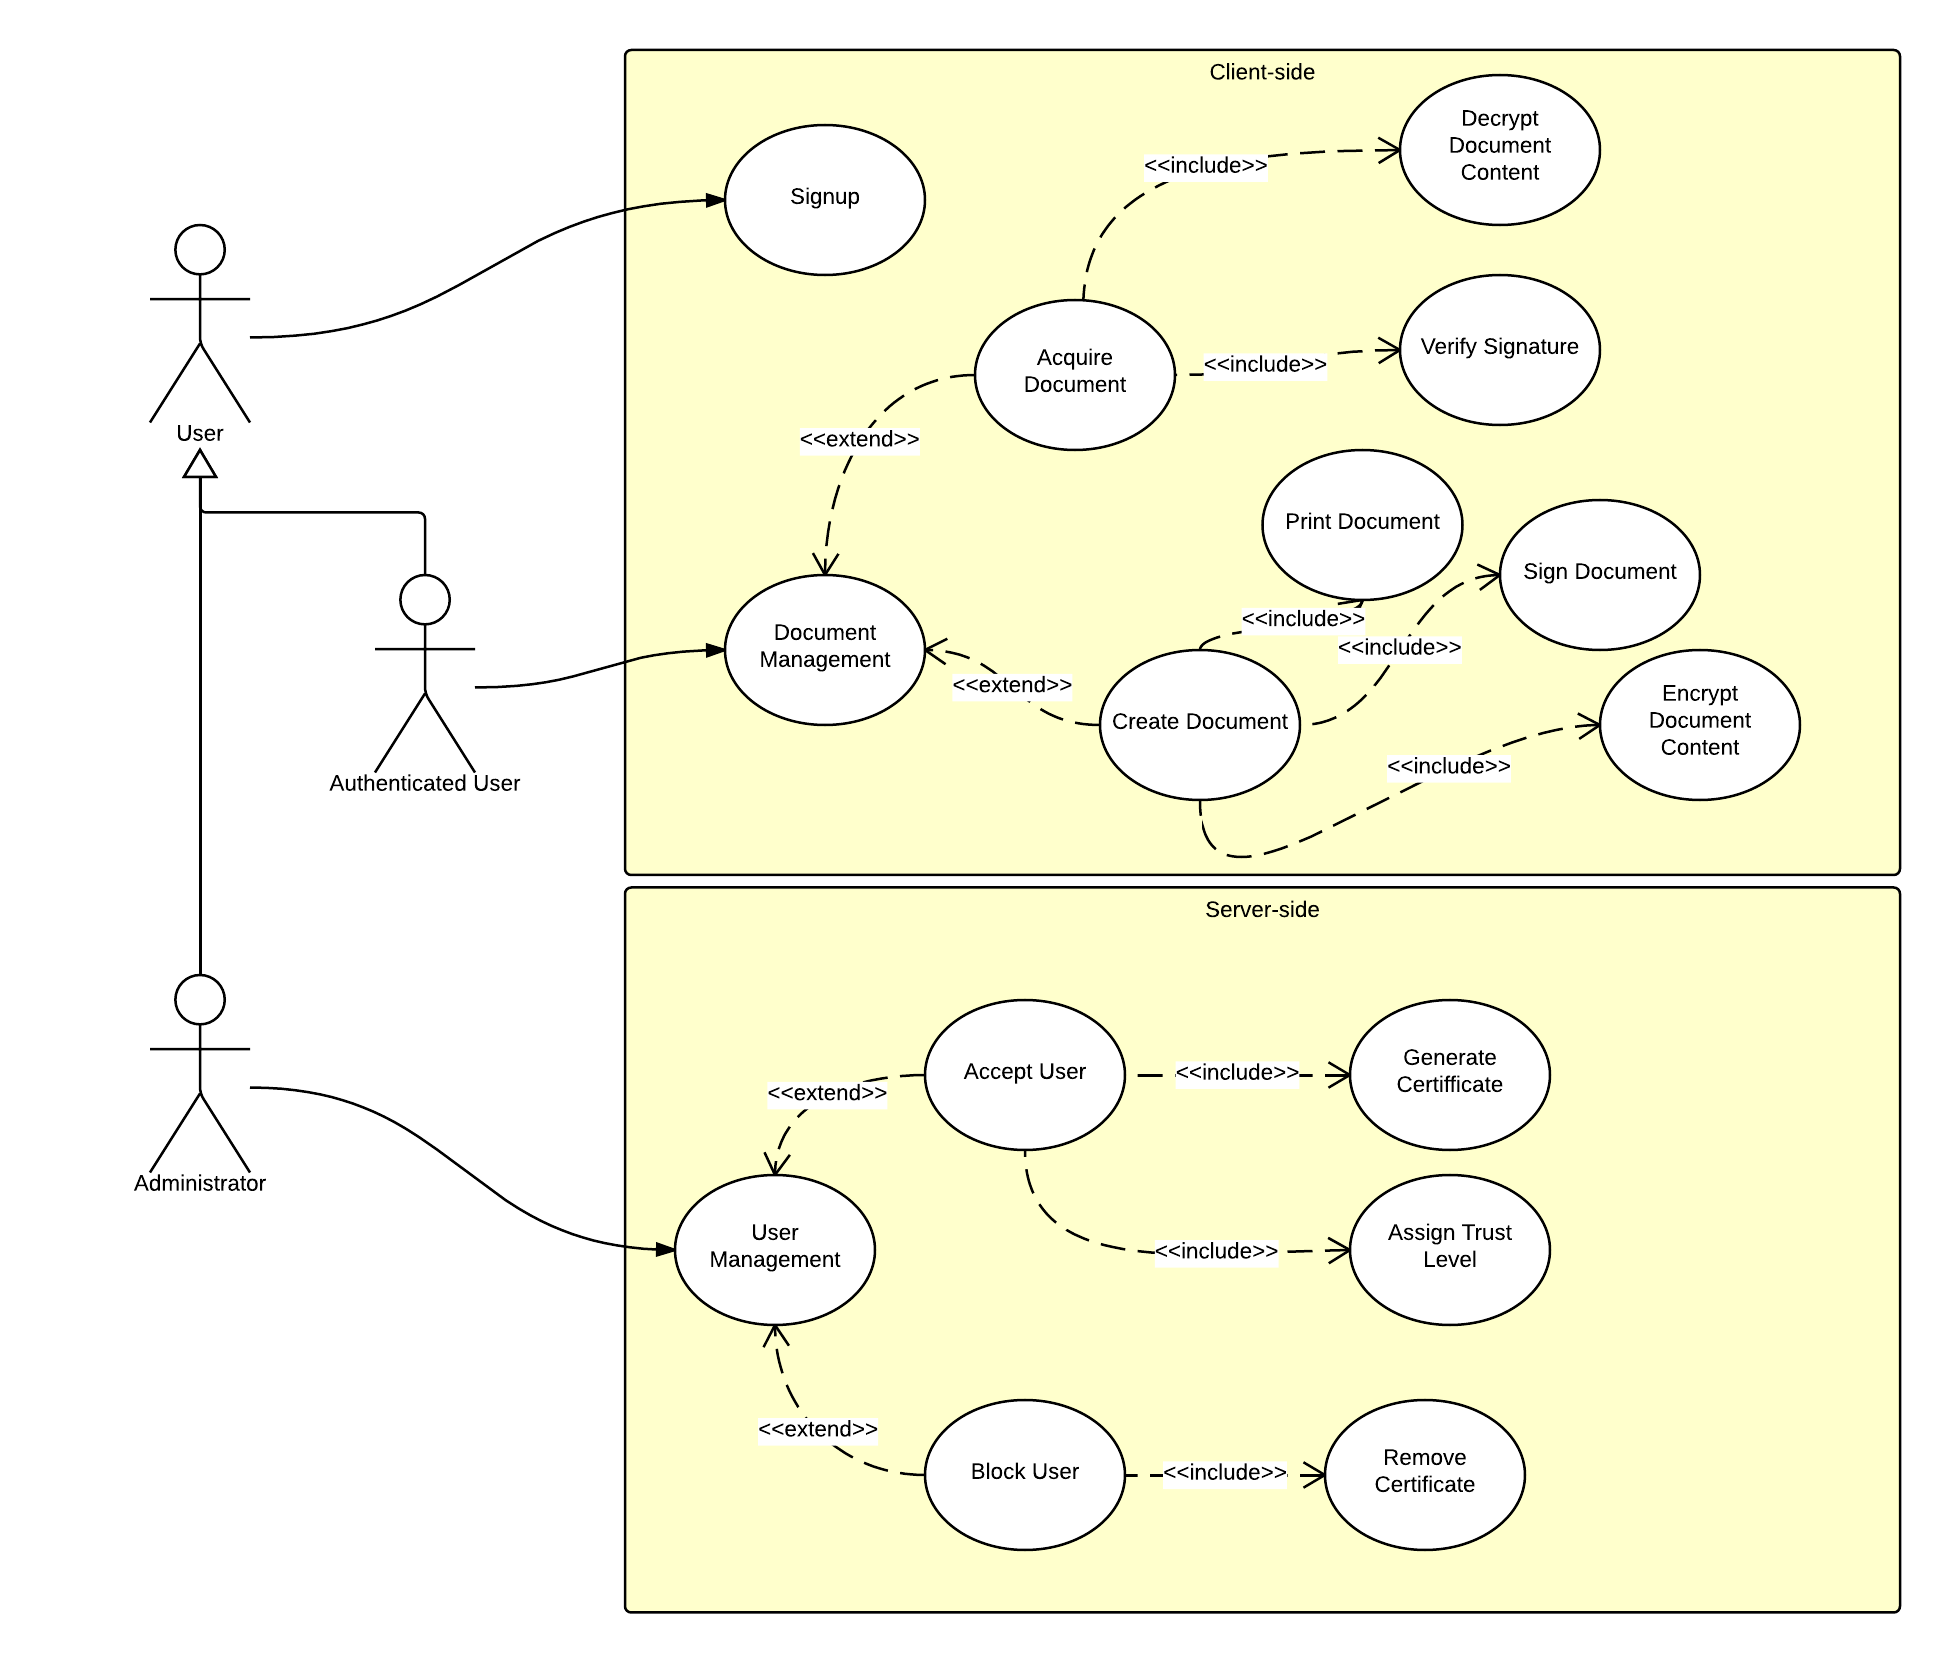
\includegraphics[scale=0.9]{Immagini/usecase}
		\caption[Use Case Diagram]{Diagramma dei casi d'uso del sistema software realizzato}
		\label{fig:usecase}
		\end{figure}
	\end{center}
La prima cosa che va evidenziata è che il tutto è strutturato secondo un architettura di tipo client/server. Questi due componenti dialogano tra di loro utilizzando una connessione sicura basata su SSL\footnote{Dettagli maggiori saranno dati nel paragrafo~\ref{sec:sicurezza}.}. Da quello che si può evincere, il server è un componente fondamentale che espone la funzionalità di \emph{provisioning} delle chiavi. Esso mantiene sia le chiavi di livello necessarie per la cifratura del documento, sia le chiavi pubbliche degli utenti registrati al sistema.

Da quello che si può vedere dalla figura~\ref{fig:usecase} nel sistema si hanno 3 attori importanti: l'amministratore, l'utente registrato (autenticato) e l'utente semplice che non ha mai utilizzato il sistema.
Come è stato già detto, l'amministratore si occupa di gestire l'accesso degli utenti. Questo vuol dire che ha piena facoltà di abilitare gli utenti all'utilizzo del sistema verificandone l'identità con procedure interne all'azienda che possono variare di caso in caso e che esulano completamente dagli scopi di questo progetto.
Oltre a questo può decidere di limitare l'accesso al sistema bloccando l'utente con una semplice procedura, grazie alla quale il server è in grado di comprendere se l'utente che si connette è autorizzato oppure no ad ottenere le chiavi di un certo livello.
Altro compito fondamentale è quello dell'assegnazione del Trust~Level che viene deciso in fase di abilitazione dell'utente al sistema. Tuttavia questo può essere anche cambiato successivamente. Grazie al Trust~Level, l'utente sarà abilitato a conoscere solo i segreti per cui è stato autorizzato, quindi l'assegnazione di questo parametro è fondamentale e richiede la massima attenzione.

L'utente registrato (o come riportato in figura~\ref{fig:usecase} ``autenticato'') rappresenta una qualsiasi persona che è stata abilitata dall'amministratore ad usare l'applicazione in tutte le sue funzionalità attuali. Un utente di questo tipo dispone di una coppia di chiavi asimmetriche RSA a $1024$ \texttt{bit} e di un certificato \texttt{X.509} che viene utilizzato per le connessioni al server che richiedono mutua autenticazione. L'utente autenticato ha la possibilità di comporre un documento, oscurarlo in alcune sue parti utilizzando le chiavi di livello a cui può accedere, e firmarlo con la propria chiave privata RSA. 
Naturalmente oltre alla composizione del documento, l'utente registrato ha anche la facoltà di leggere quello che è stato inviato a lui o agli utenti con il suo stesso Trust~Level\footnote{Si rimanda al paragrafo~\ref{sec:sicurezza} per una trattazione più approfondita di questo aspetto.}.

Per quanto riguarda l'utente semplice, si è sicuramente notato che questo ha l'unica facoltà di registrarsi al sistema. Questo perché non dispone ancora di un certificato da usare per l'autenticazione e quindi non ha alcuna possibilità di leggere le informazioni se non provando ad eseguire un attacco sulla sicurezza del sistema o del documento cartaceo.

\section{Architettura}
	\label{sec:architettura}
Data una panoramica dei requisiti e delle funzionalità principali del sistema, si passerà adesso ad analizzare più in dettaglio l'architettura del sistema realizzato.
	\begin{center}	
		\begin{figure}[H]
		\centering
		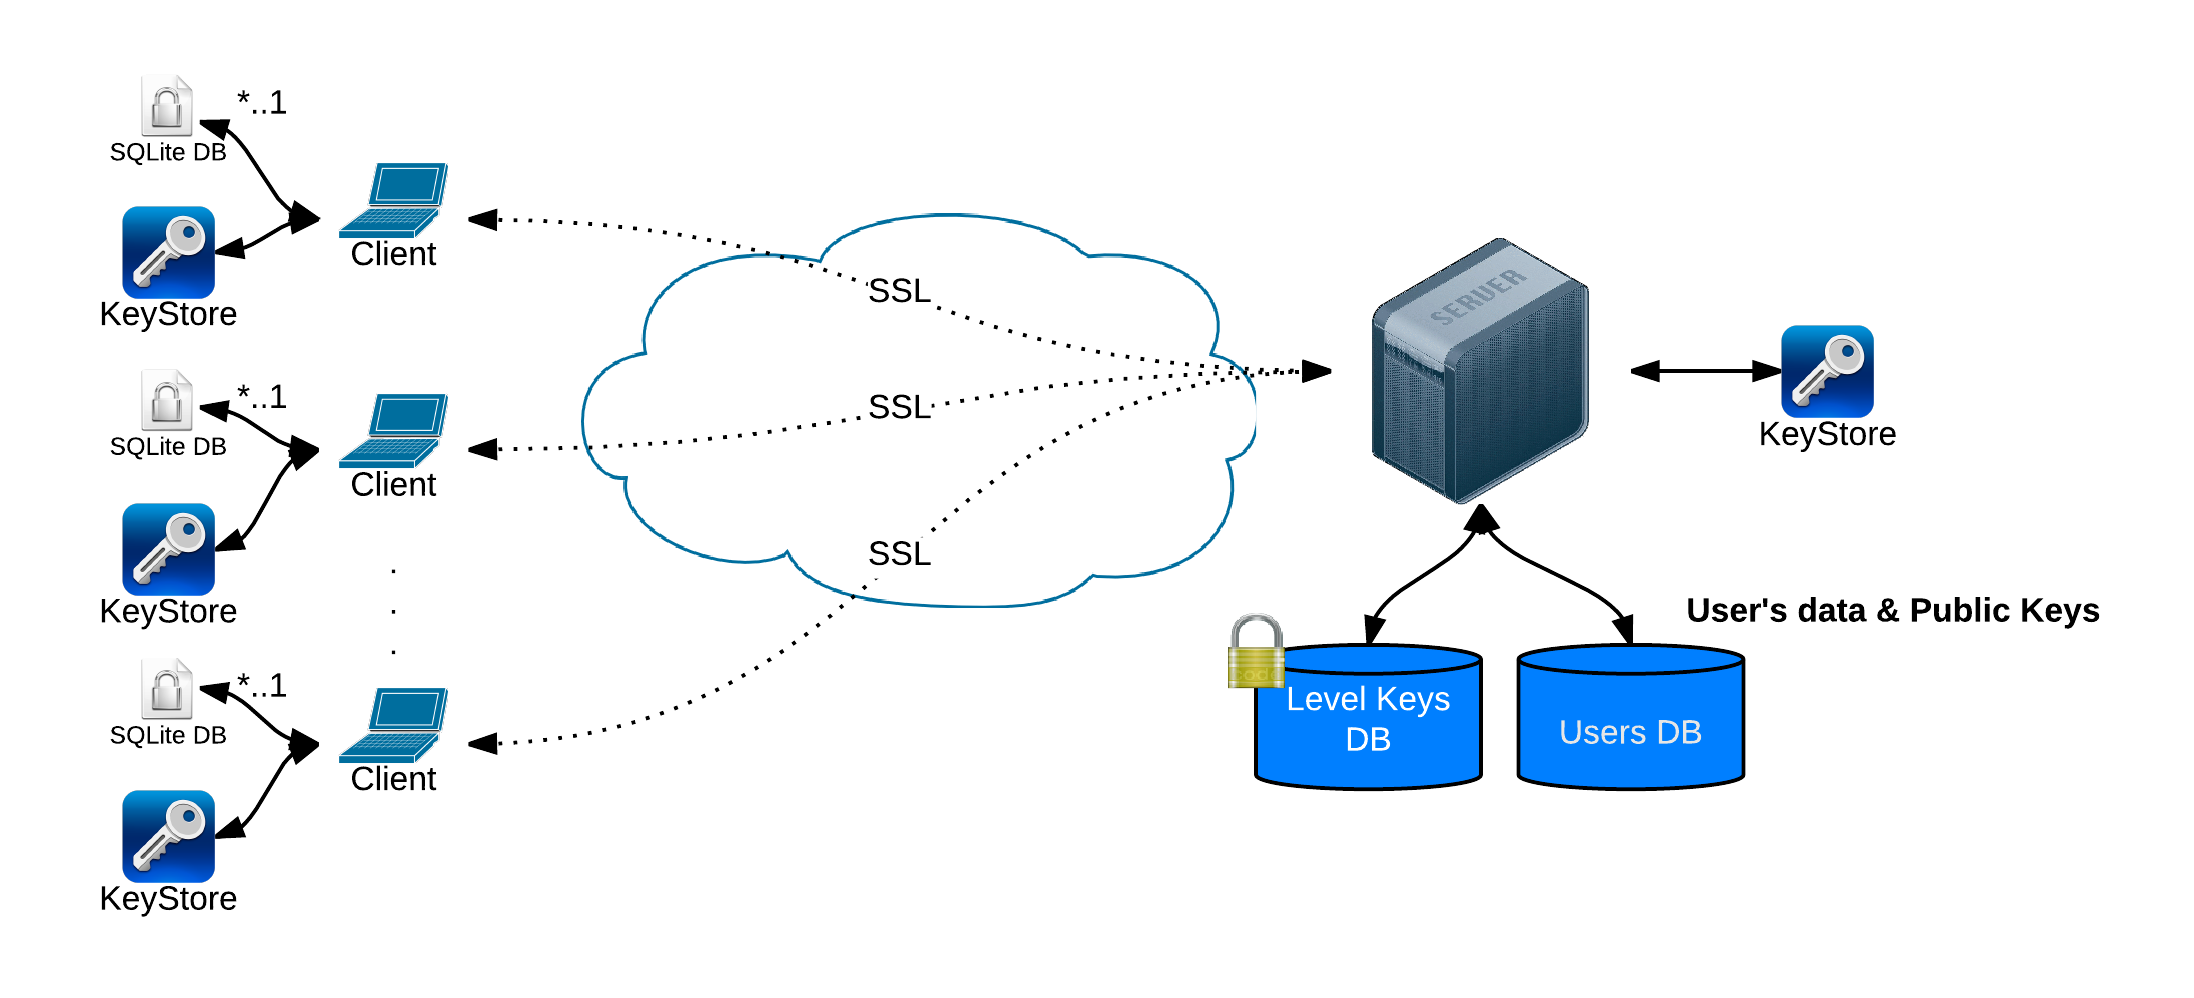
\includegraphics[scale=0.9]{Immagini/architettura}
		\caption[Architettura del sistema]{In questa figura sono rappresentate le componenti del sistema software realizzato.}
		\label{fig:architettura}
		\end{figure}
	\end{center}
Quella mostrata in figura~\ref{fig:architettura} è l'architettura del sistema che è stato realizzato per questo progetto.
Come si può vedere (anche da quanto già accennato nei paragrafi precedenti) il sistema si compone di due applicazione separate: un server e un client.
Entrambe queste applicazioni comunicano con il protocollo TCP/IP con l'aggiunta del layer di sicurezza realizzato da SSL.

Per quanto riguarda il server esso offre $2$ servizi differenti. Il primo (sulla porta $8888$) che richiede che gli utenti in connessione confermino la loro identità inviando il loro certificato così come previsto dallo standard SSL quando il server richiede, come requisito nella fase di handshake, il certificato del client al fine di verificare la mutua autenticazione.
Le funzionalità offerte da questo primo servizio sono:
\begin{itemize}
	\item fornire le chiavi~di~livello agli utenti autenticati che le richiedono (purché ne abbiano diritto in base al loro livello~di~fiducia);
	\item fornire le chiavi pubbliche degli utenti registrati al sistema, così che gli utenti possano verificare le firme digitali apposte sui documenti cartacei.
\end{itemize}
Il secondo servizio (sulla porta $8889$) non richiede invece autenticazione mutua, in quanto è quello che permette agli utenti nuovi di comunicare i loro dati al server al fine di richiedere un'abilitazione all'utilizzo del sistema.

Da come si può vedere in figura~\ref{fig:architettura} il server dispone di una connessione a due database MySQL separati e ad un \emph{Java~KeyStore}\footnote{Un Java~KeyStore (JKS) è un repository di certificati pubblici e chiavi utilizzato per la cifratura dei pacchetti su connessioni SSL.}. 
Il KeyStore serve a memorizzare i certificati degli utenti, in modo che possano essere identificati univocamente nella fase di handshake della connessione.
Il primo dei due database si occupa di gestire le chiavi di livello necessarie per la cifratura del documento. Le chiavi sono memorizzate cifrate con \textbf{AES} tramite una chiave robusta e ad ognuna di queste è associato il livello di fiducia relativo. L'altro database si occupa di mantenere le informazioni degli utenti registrati, comprese le loro rispettive chiavi pubbliche. Si è deciso di separare i due database in quanto essi devono soddisfare requisiti di sicurezza differenti in quanto dalla segretezza delle chiavi di livello (che dovrebbero essere cambiate periodicamente) dipende la robustezza dell'intero sistema di cifratura dei documenti. La separazione permetterebbe allora di ospitare su server differenti i due database, che sarebbero quindi protetti con password robuste e differenti e con l'aggiunta di altri sistemi di sicurezza, quali \emph{VPN} e \emph{Firewall}, per la protezione da attacchi esterni.

All'applicazione stand-alone lato client compete invece tutta la gestione dei documenti, ossia la cifratura, la firma e la decifrazione delle immagini. Dal diagramma dell'architettura si vede come anche questo componente presenti una connessione ad un KeyStore e a diversi database di tipo SQLite. Per quanto riguarda il KeyStore, questo assolve alla stessa funzione di quello del server, ossia mantiene il certificato pubblico del server e la chiave privata di ciascun utente insieme al suo rispettivo certificato. Ogni entry del KeyStore (che nella pratica non è altro che una mappa indicizzata per una stringa chiamata \emph{alias}) è cifrata con la password personale di ciascun utente. In più anche il file del KeyStore stesso è cifrato con una master key.
I database SQLite, invece, servono a memorizzare i dati locali di ciascun utente compresa anche la coppia di chiavi asimmetriche RSA. Ogni utente ha il proprio database personale cifrato con la sua password.
Il motivo di questa scelta riguarda soprattutto il fatto che i database SQLite non sono altro che file binari che sono gestiti da un software molto leggero (dimensioni nell'ordine delle centinaia di KiloByte). Quindi possono essere manipolati molto meglio rispetto per esempio ad un file di configurazione personalizzato per cui si sarebbe dovuta implementare una logica di gestione.
Quindi la facilità di gestione e la leggerezza sono stati i principali responsabili di questa scelta.

\section{Focus sulla sicurezza}
	\label{sec:sicurezza}
Dopo aver trattato in dettaglio l'architettura del sistema, si può passare a descrivere tutte le procedure che sono state implementate per gestire la sicurezza del sistema e dei documenti cartacei. Di seguito i dettagli riguardanti la sicurezza.

\subsection{Autenticazione}
	\label{subsec:autenticazione}
Come già detto nei paragrafi precedenti, per funzionare in modo sicuro, il sistema ha bisogno che gli utenti che lo utilizzano siano ben noti. Questo significa che ogni utente deve disporre di un certificato che comunichi la sua identità. Infatti, il requisito più importante per stabilire una comunicazione con il server per ottenere chiavi è l'autenticazione del client nella fase di handshake della connessione SSL.
Affinché sussista la mutua autenticazione il server deve però conoscere già a priori il certificato del client. E allo stesso modo anche il client deve conoscere il certificato del server.
Nel caso di questo progetto, si è deciso di mettere da subito a disposizione del client il certificato del server come configurazione di base. In questo modo si è sicuri che da subito l'applicazione client inizierà a parlare con il server certificato.
Tuttavia lo stesso non può essere fatto dalla parte del server, in quanto questo non può conoscere a priori tutti i possibili utenti che entreranno nel sistema. Quindi si è deciso di prevedere una procedura di registrazione nella quale il risultato finale è il rilascio all'utente di un certificato autenticato dal server che a sua volta lo aggiungerà nel proprio KeyStore.
Da osservare il fatto che nella fase di registrazione l'utente dialogherà col server senza comunicare la sua identità. \accg{E} per questo che si è resa necessaria la figura dell'\textbf{amministratore} che si occuperà di verificare la reale identità dell'utente durante questa fase critica, ed eventualmente lo abiliterà ad usare il sistema.
	\begin{center}	
		\begin{figure}[H]
		\centering
		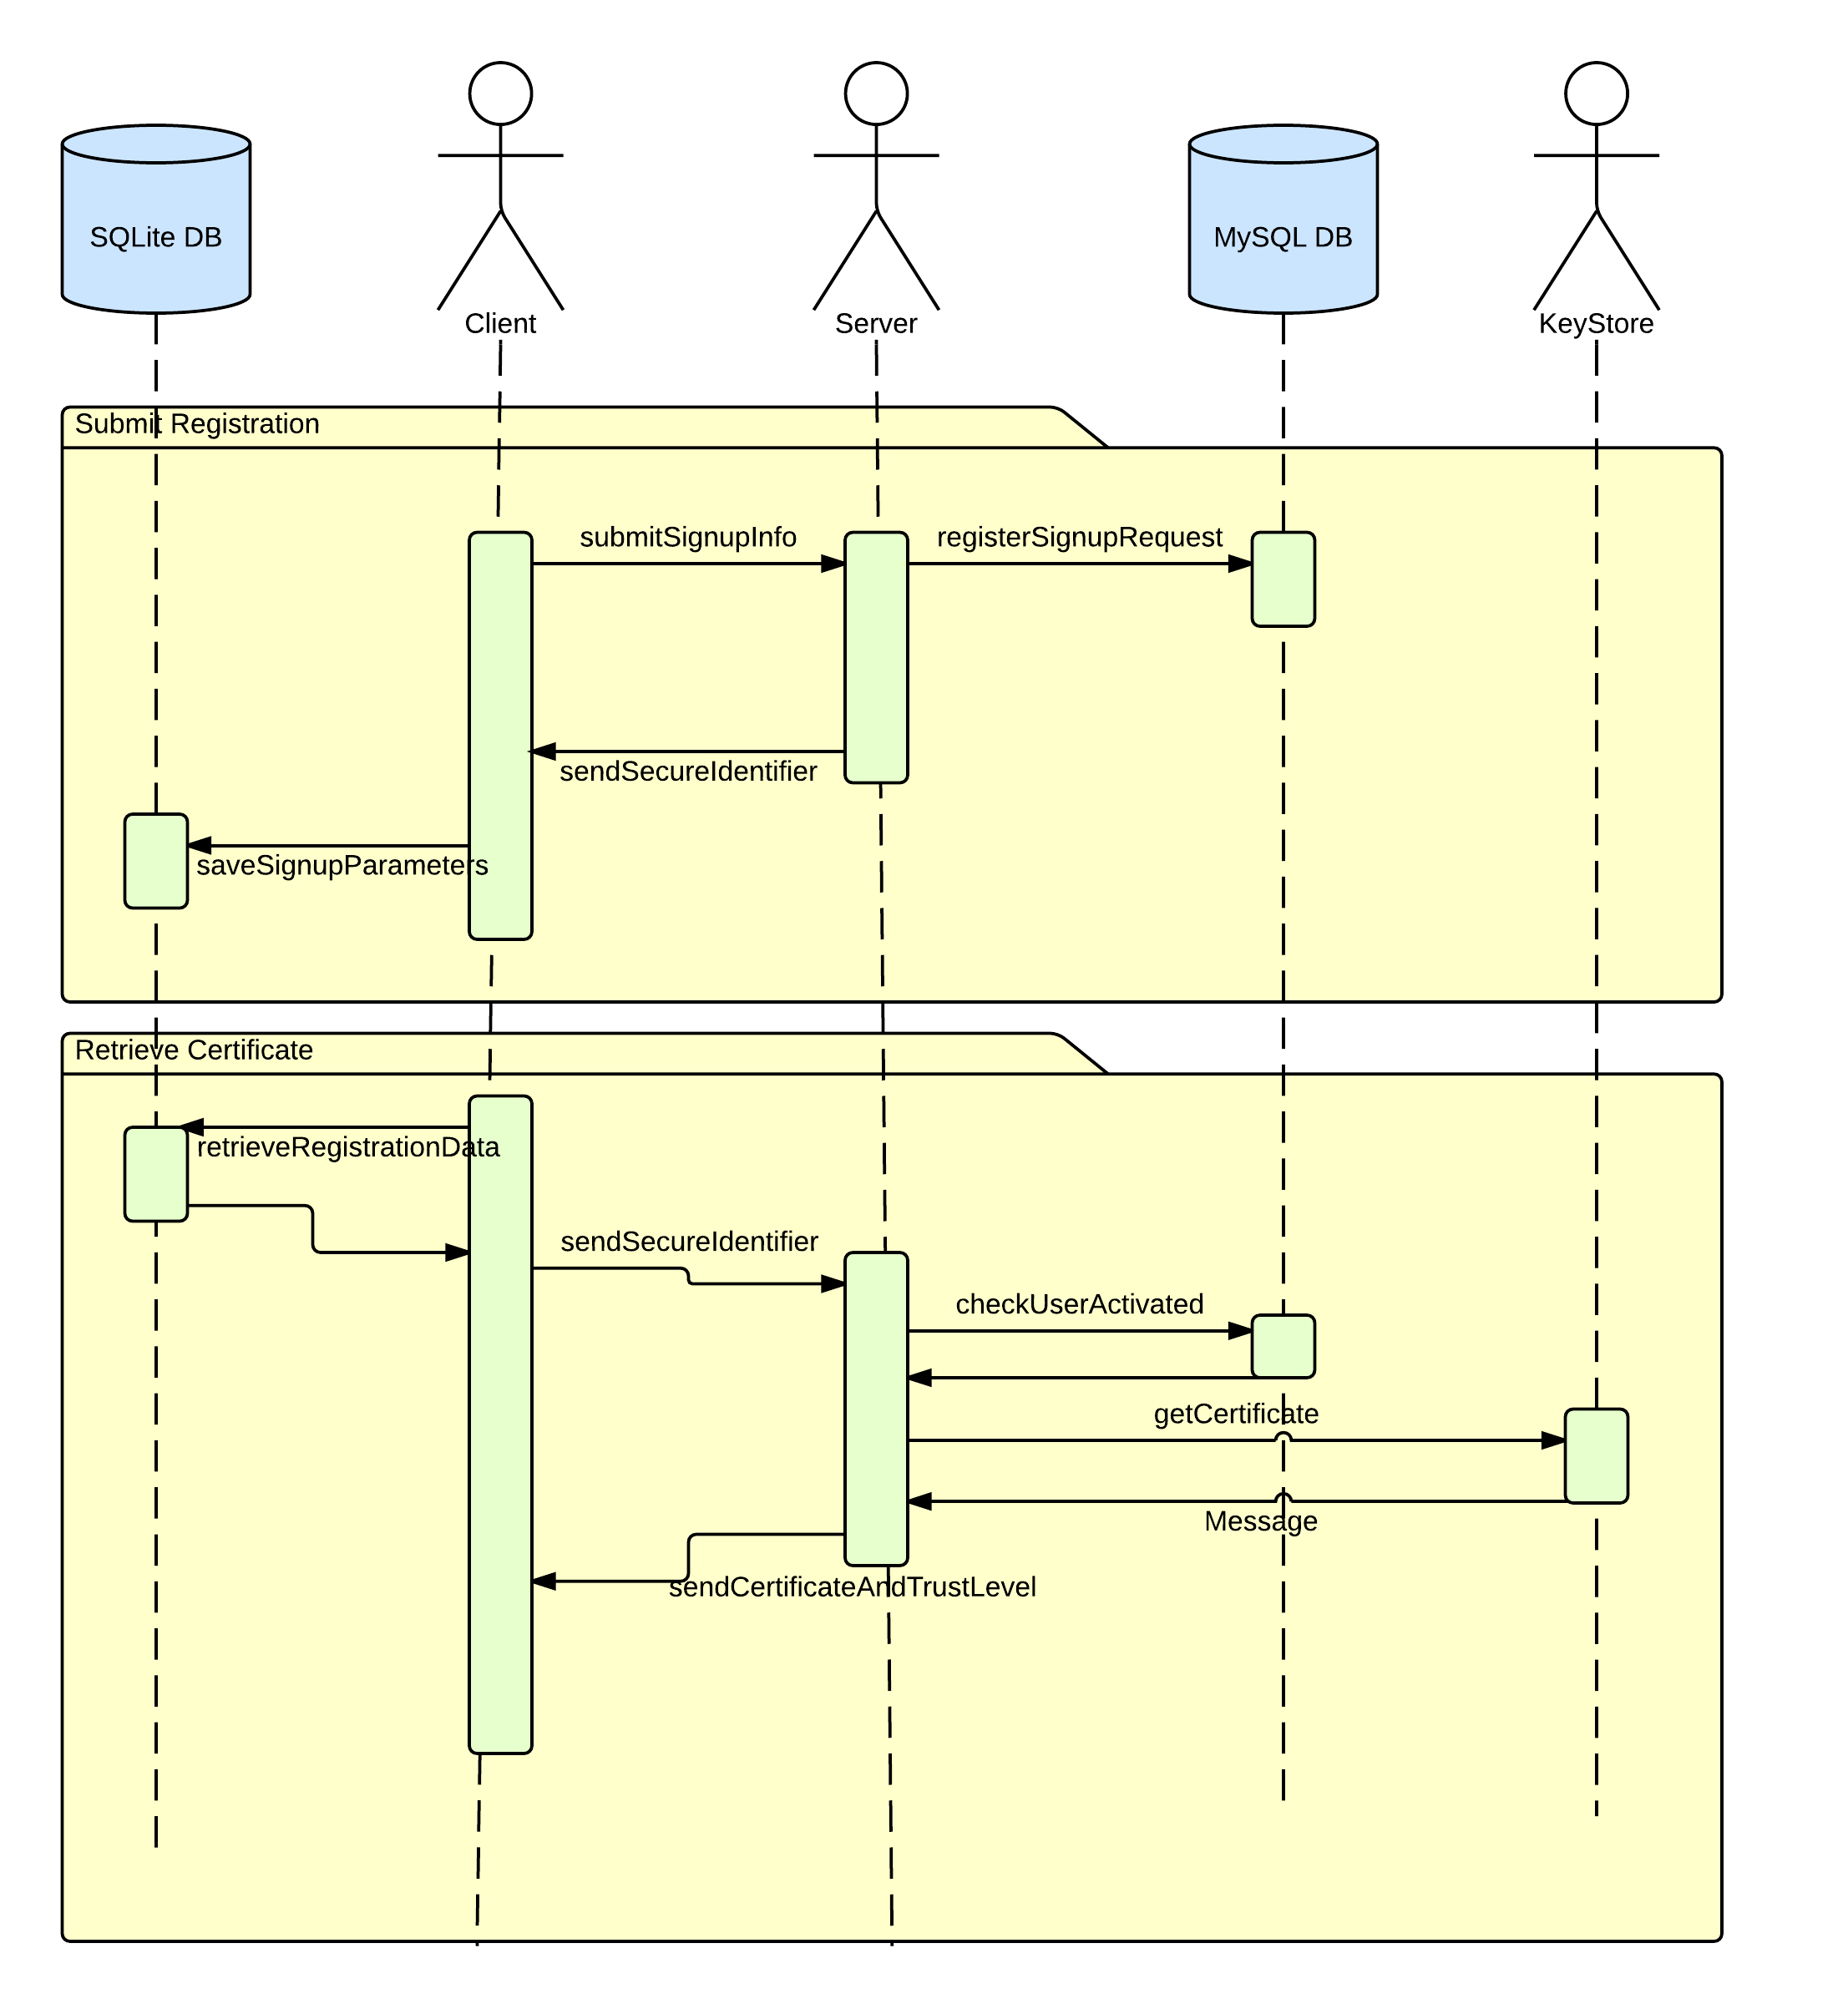
\includegraphics[scale=0.7]{Immagini/signup}
		\caption[Sequence Diagram: Registrazione al Sistema]{Diagramma di sequenza rappresentante le due fasi principali della registrazione al sistema}
		\label{fig:registrazione}
		\end{figure}
	\end{center}
La fase di registrazione, i cui passi principali sono illustrati nel diagramma di sequenza in figura~\ref{fig:registrazione}, è composta di due fasi. Nella prima fase il nuovo utente comunica al server autenticato le proprie credenziali (nome, cognome, chiave pubblica, organizzazione di appartenenza, città e paese di residenza) che vengono salvate nel database in attesa di elaborazione. Come risposta della presa in consegna della richiesta, il server genera un token univoco (\textbf{SecureID}) che successivamente il client può utilizzare per recuperare il proprio certificato e che deve essere tenuto segreto dall'utente. La fase di elaborazione viene eseguita dall'amministratore che si accerta che i dati sottomessi dall'utente siano corretti e veri. A questo punto, l'amministratore ha due possibilità: abilitare l'utente all'uso del sistema oppure respingere la sua domanda.
Nel secondo caso non avverrà nulla e l'utente verrà informato al successivo accesso che la sua richiesta è stata respinta. Nel caso in cui invece la richiesta venga accolta, viene generato un certificato utilizzando le credenziali e la chiave pubblica dell'utente e firmato utilizzando la chiave privata del server. Questo farà sì che il server possa stabilire in un secondo momento l'autenticità del certificato e capire quindi se è stato emesso da lui oppure no (decisione importante per capire se l'utente può accedere alle varie funzionalità). Successivamente il certificato generato viene salvato nel KeyStore del server.
Nella seconda fase (corrispondente al blocco in basso in figura~\ref{fig:registrazione}) l'utente utilizza il \textbf{SecureID} per recuperare il proprio certificato. Da quel momento in poi potrà utilizzare a pieno tutte le funzionalità del sistema compatibilmente con il \textbf{livello~di~fiducia} assegnato.

%parte di pasquale (rivedila tu bene)
Quello appena descritto è ciò che avviene dal punto di vista del server. Per quanto riguarda l'applicazione client, la procedura di registrazione prepara all'utente l'ambiente per l'utilizzo del sistema. In particolare vengono generate directory dedicate dove verranno posti i dati temporanei delle elaborazioni e soprattutto il database SQLite cifrato dove sono memorizzati i dati sensibili dell'utente. Durante la registrazione inoltre viene generato un codice (diverso dal precedente \textbf{SecureID}) che l'utente utilizzerà successivamente per eseguire il login al sistema. \accg{E} stato dunque messo in piedi un login con doppia autenticazione per ridurre al minimo le probabilità di furto di identità.
	
\subsection{Composizione e lettura dei documenti}
	\label{subsec:documenti}
Si tratterà adesso l'aspetto principale di questo progetto: l'elaborazione dei documenti. Si descriveranno in modo dettagliato le procedure che sono state implementate per costruire, cifrare e decifrare i contenuti.

\subsubsection{Costruzione del documento}
In questo paragrafo verrà analizzata l'impaginazione del documento cartaceo.
	\begin{center}	
		\begin{figure}[H]
		\centering
		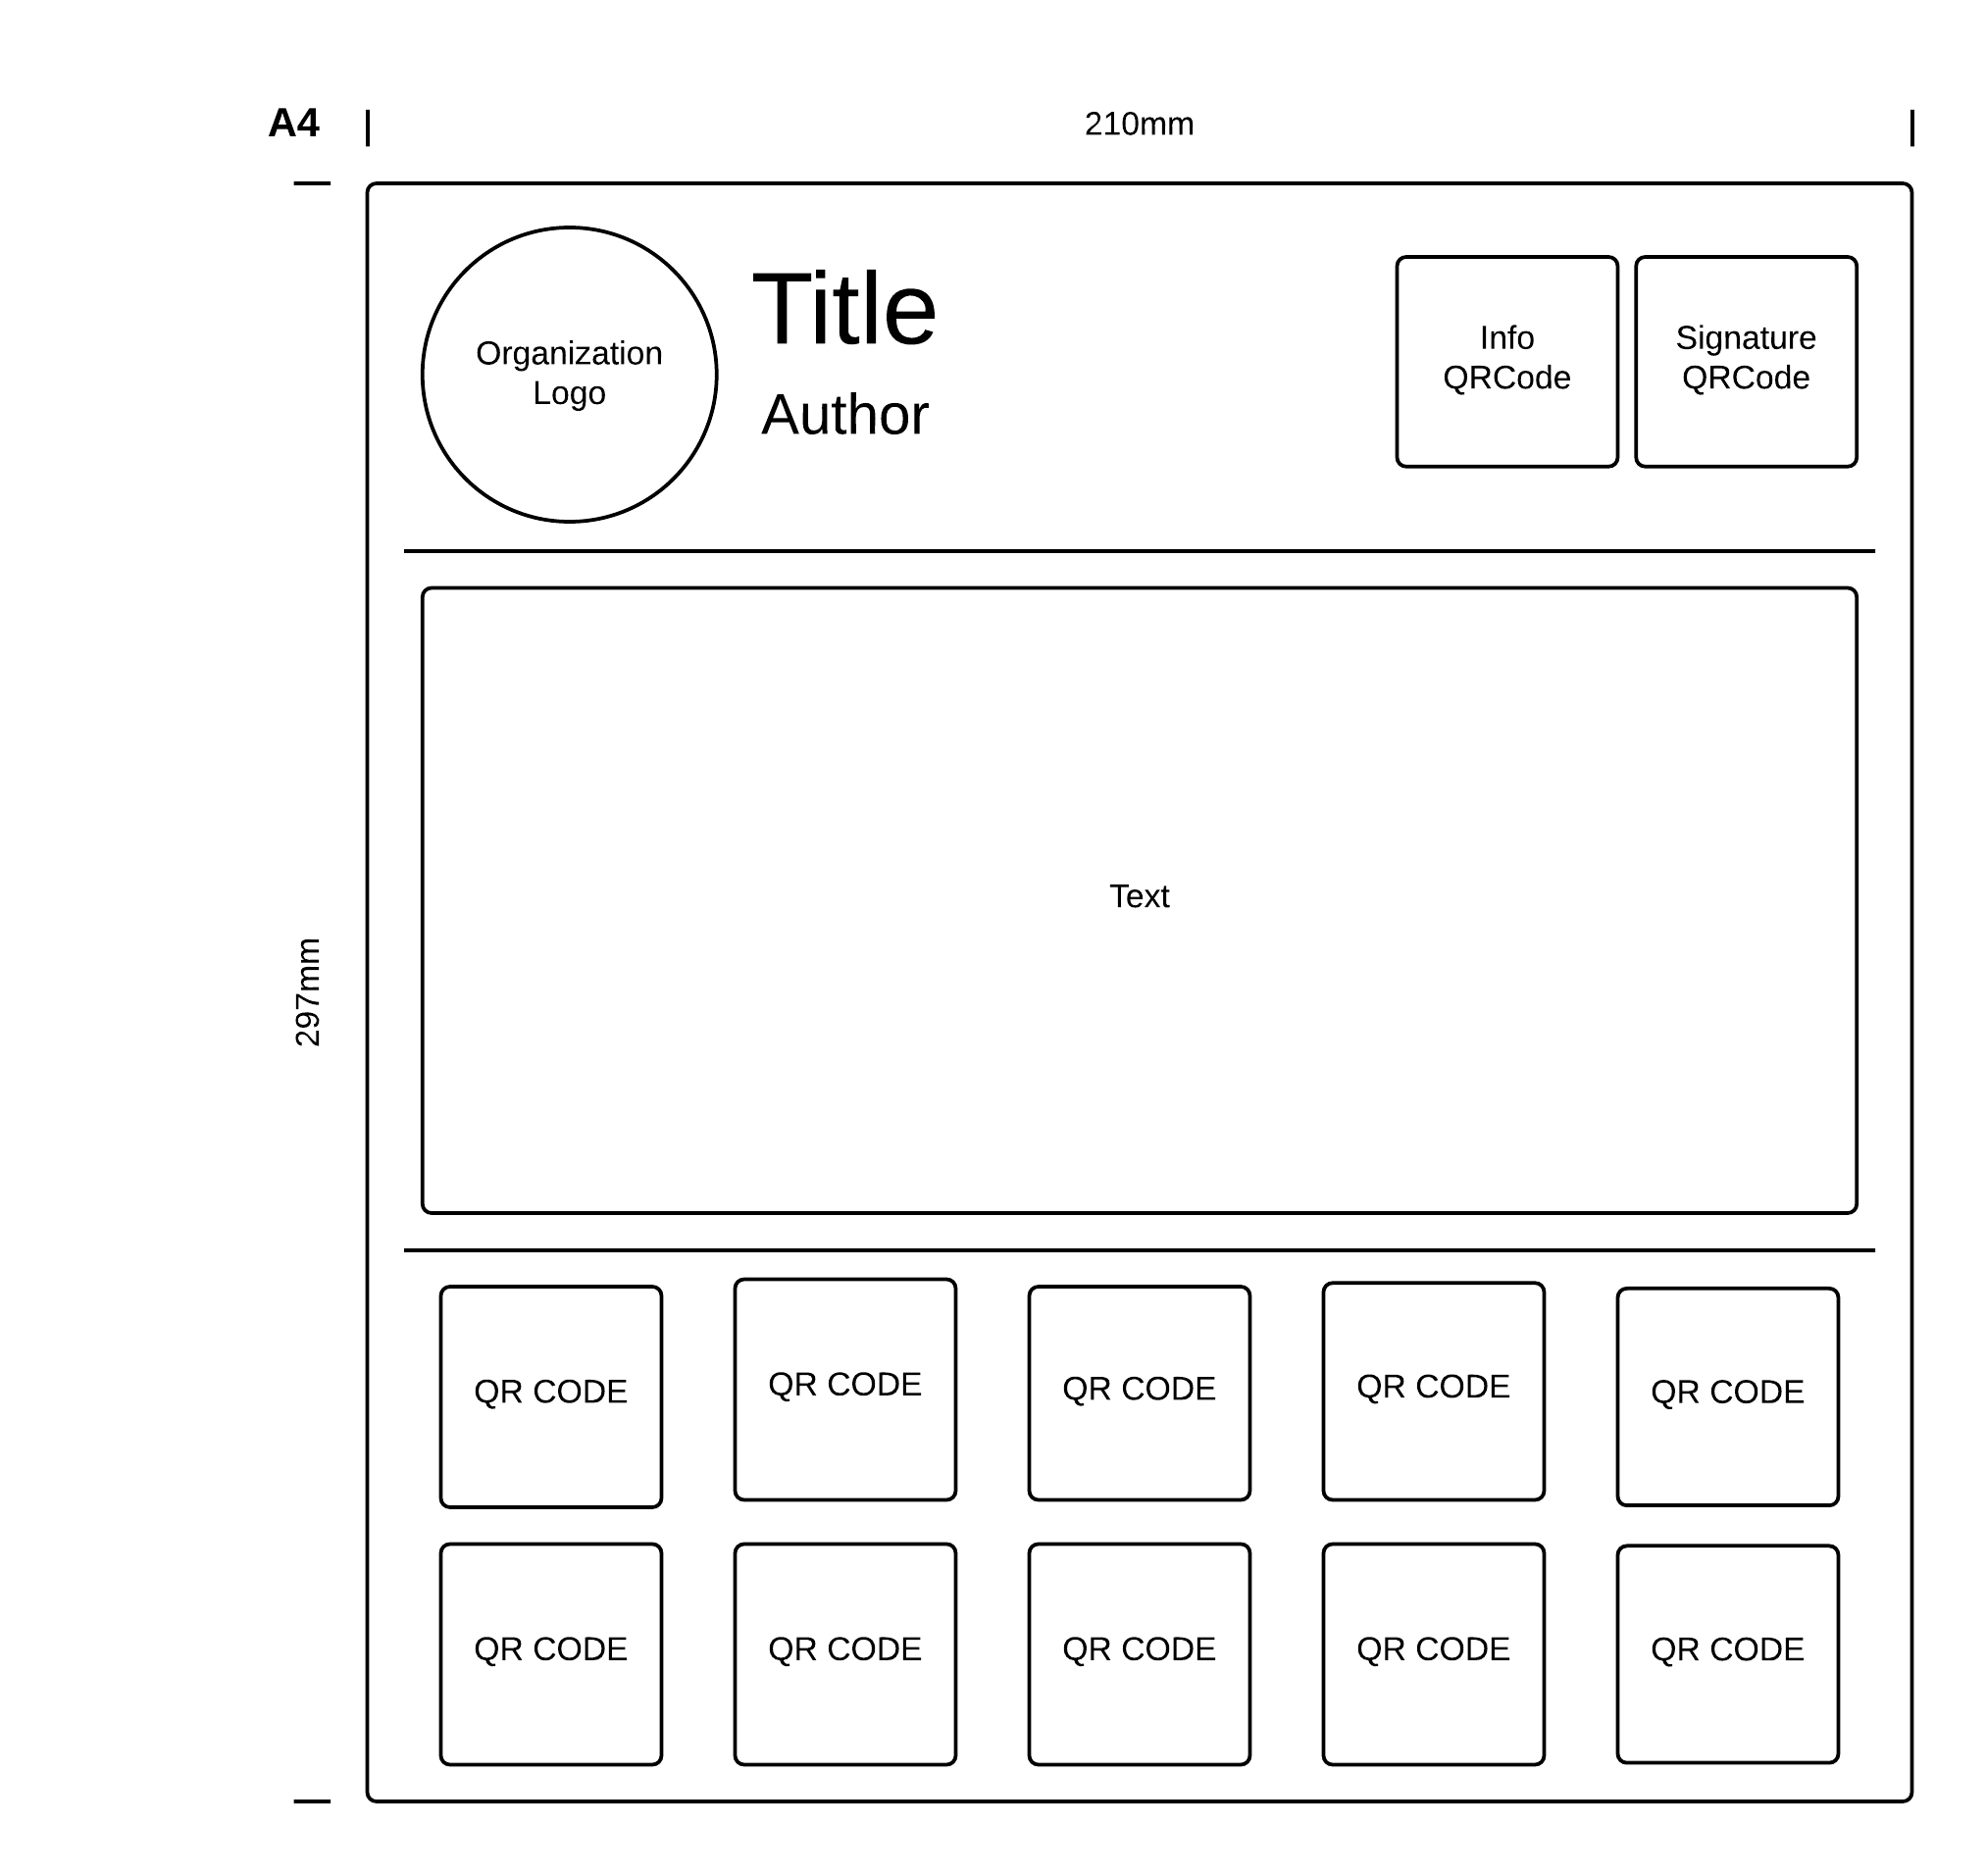
\includegraphics[scale=0.7]{Immagini/template}
		\caption[Template del documento]{Schema delle principali sezioni del documento.}
		\label{fig:template}
		\end{figure}
	\end{center}
La figura~\ref{fig:template} illustra le sezioni principali del documento. In alto si ha un'intestazione dove sono presenti un campo per il titolo, uno per l'autore e due QR-Code: in uno sarà impressa la firma dell'utente e nell'altro verranno trasportate informazioni utili a recuperare il contenuto cifrato tra cui:
\begin{itemize}
	\item titolo;
	\item mittente;
	\item UID del mittente (per consentire al destinatario di recuperare la chiave pubblica del mittente e verificare la firma);
	\item destinatario.
\end{itemize}
Nella parte centrale c'è il corpo del documento dove l'utente può inserire il testo da inviare.
Nella parte in basso vengono posizionati, infine, i QR-Code contenenti il testo cifrato e le informazioni per il posizionamento nel testo che sono anch'esse cifrate.

\subsubsection{Cifratura del Documento}

	\begin{center}	
		\begin{figure}[H]
		\centering
		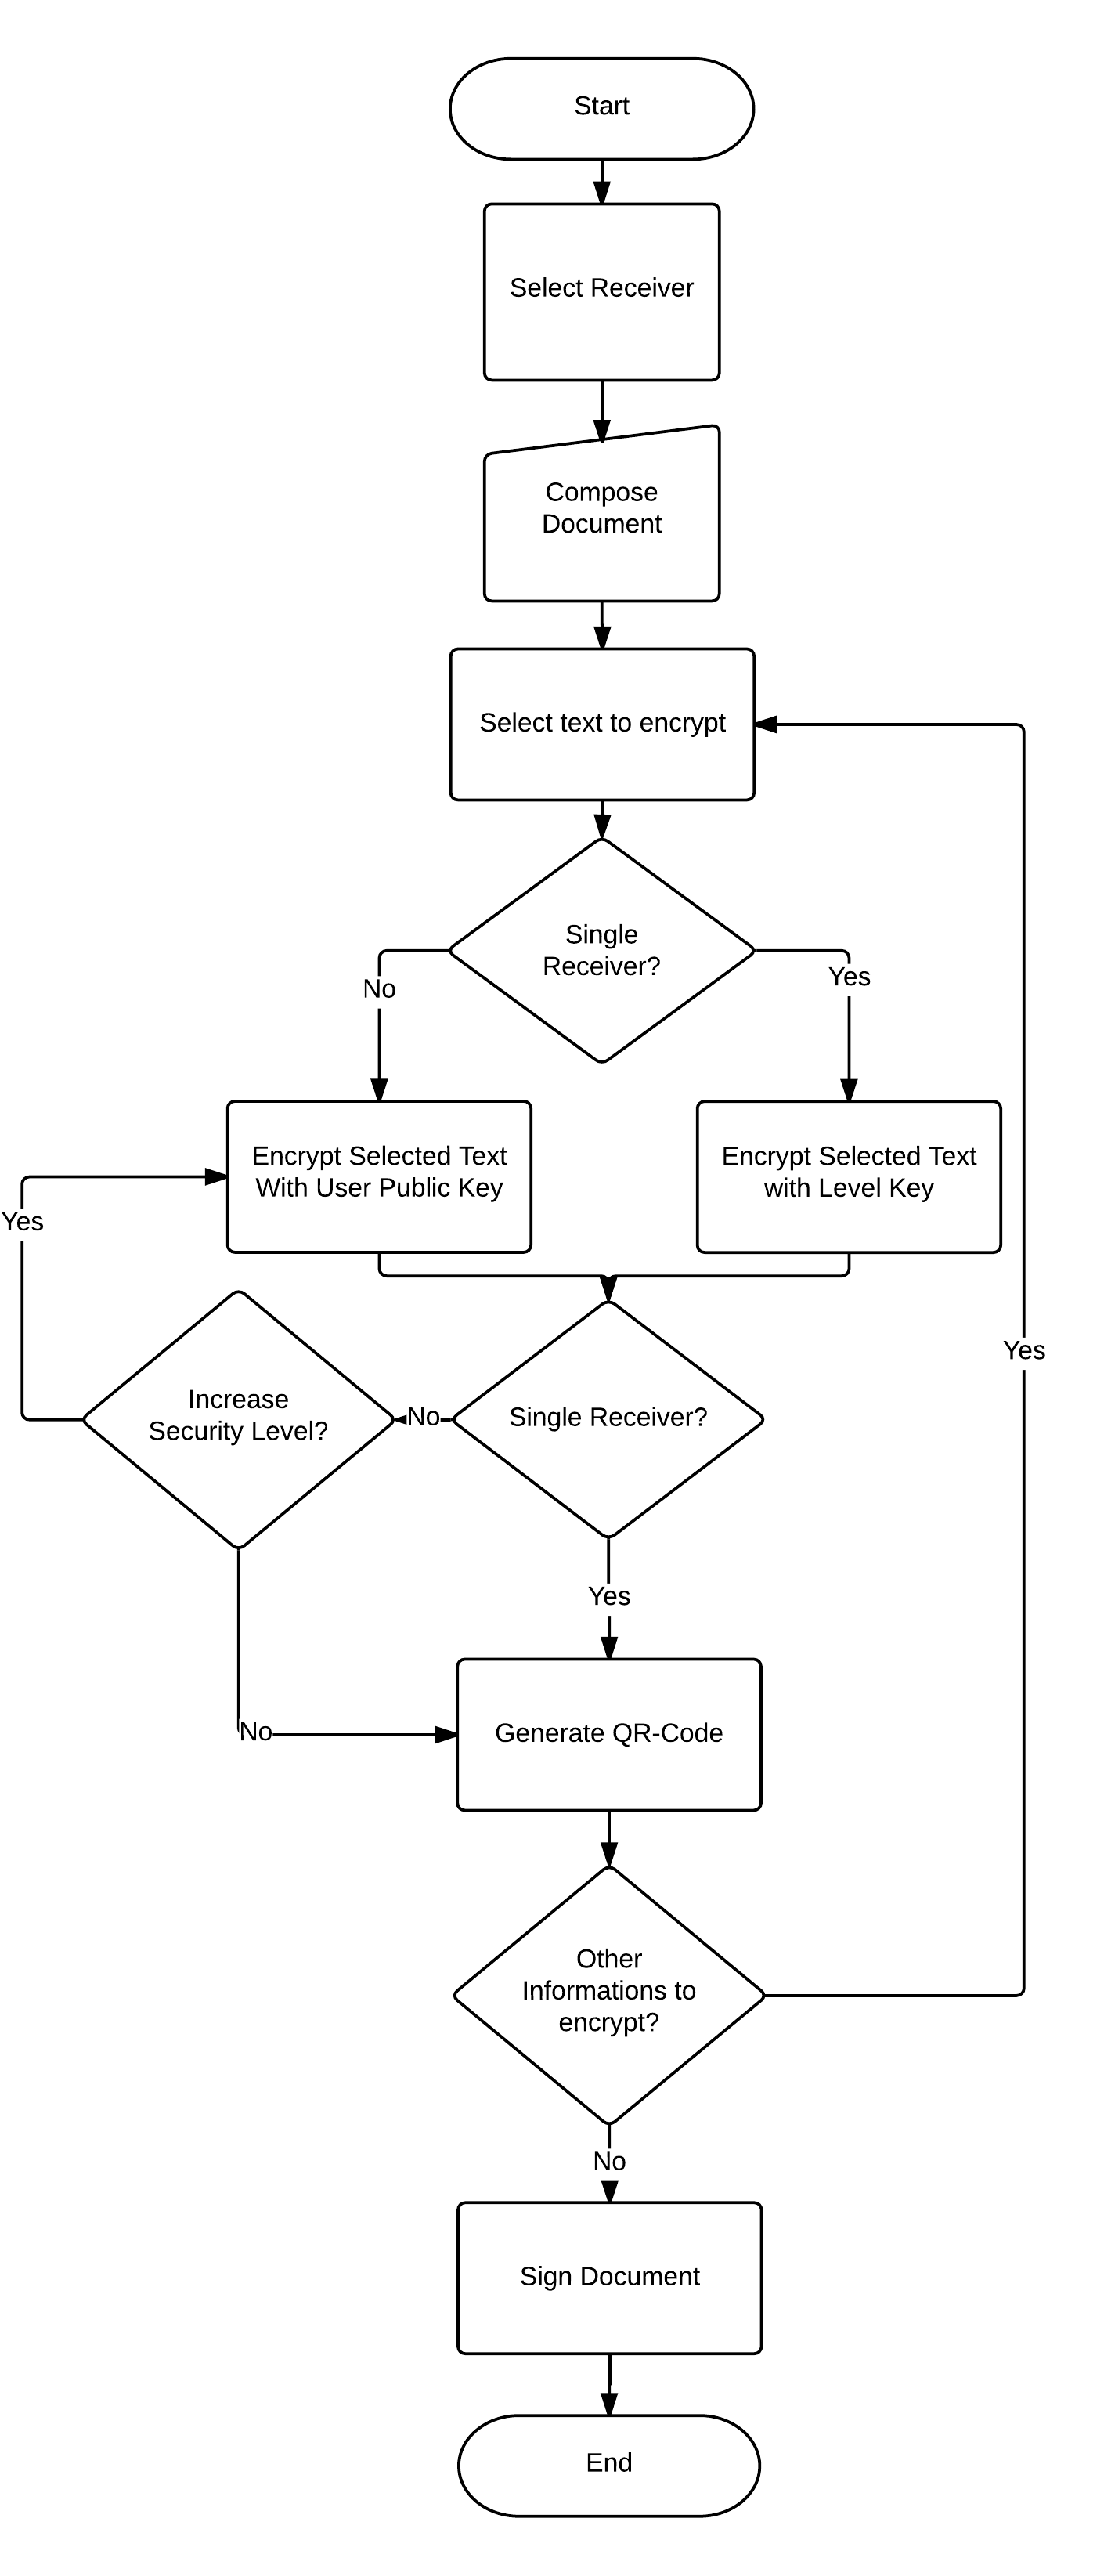
\includegraphics[scale=0.6]{Immagini/cifratura_vert}
		\caption[Flusso cifratura documento]{Diagramma di flusso per l'operazione di cifratura del documento}
		\label{fig:cifratura}
		\end{figure}
	\end{center}
\subsubsection{Decifrazione del Documento}
	\begin{center}	
		\begin{figure}[H]
		\centering
		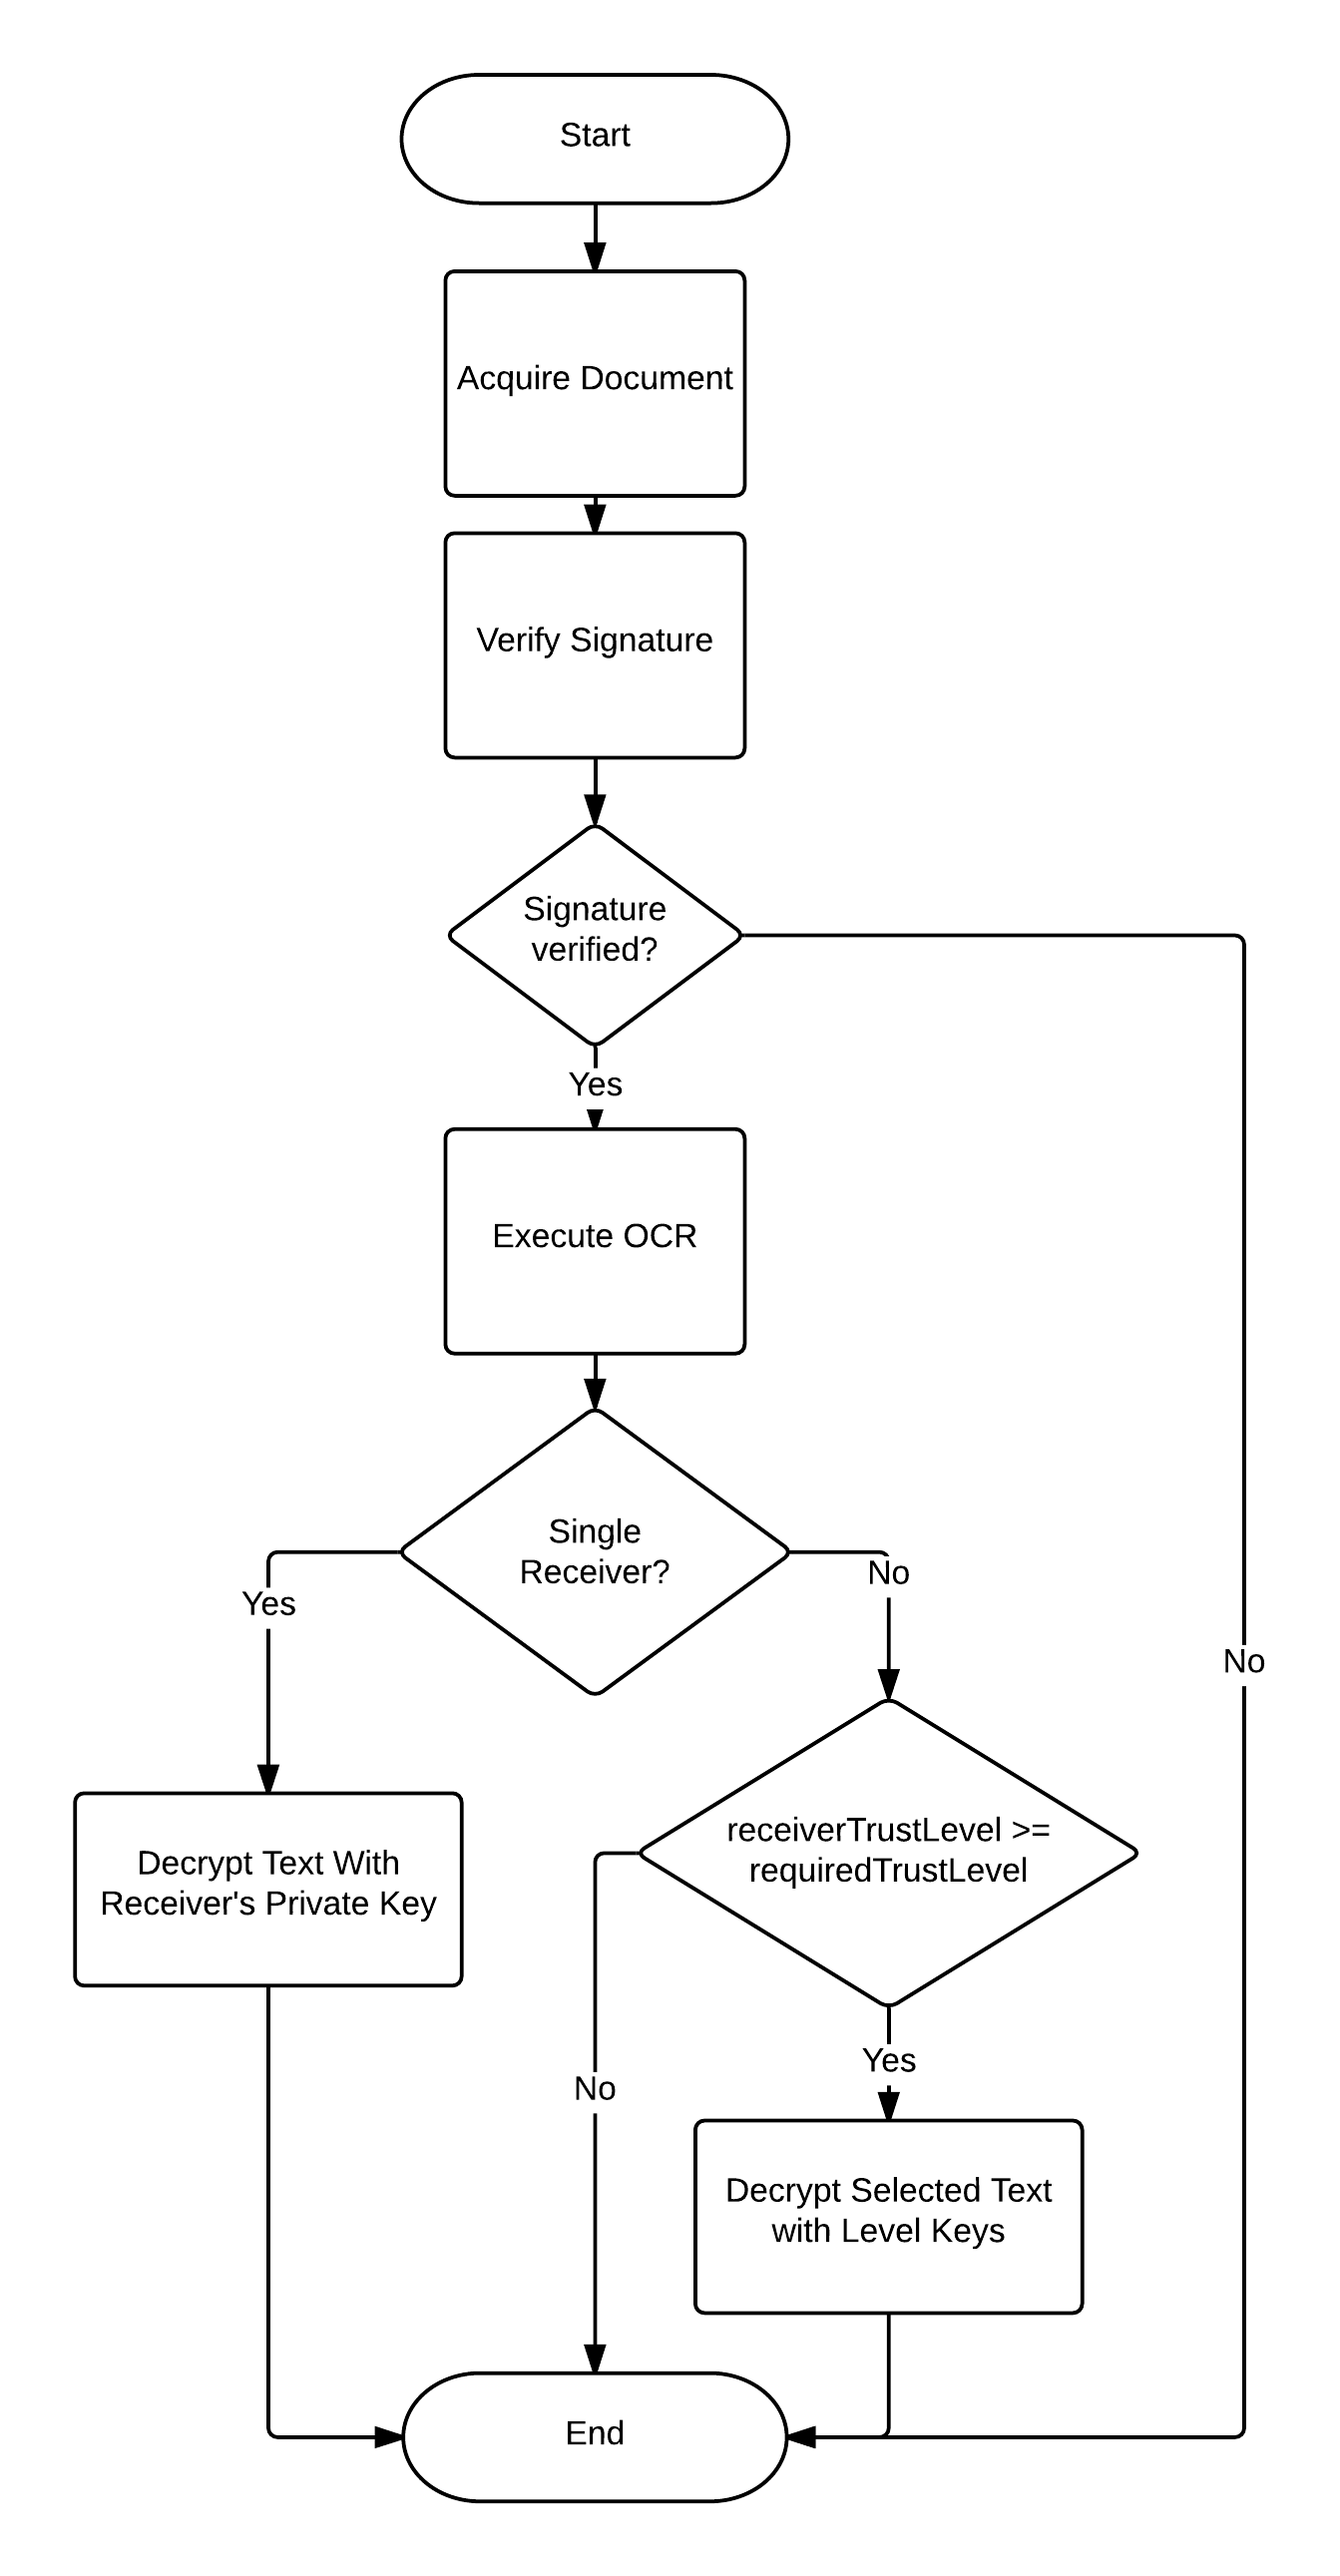
\includegraphics[scale=0.6]{Immagini/decifrazione_vert}
		\caption[Flusso decifrazione documento]{Diagramma di flusso per l'operazione di decifrazione del documento}
		\label{fig:decifrazione}
		\end{figure}
	\end{center}